\chapter{Psalm 13}

\begin{figure}
  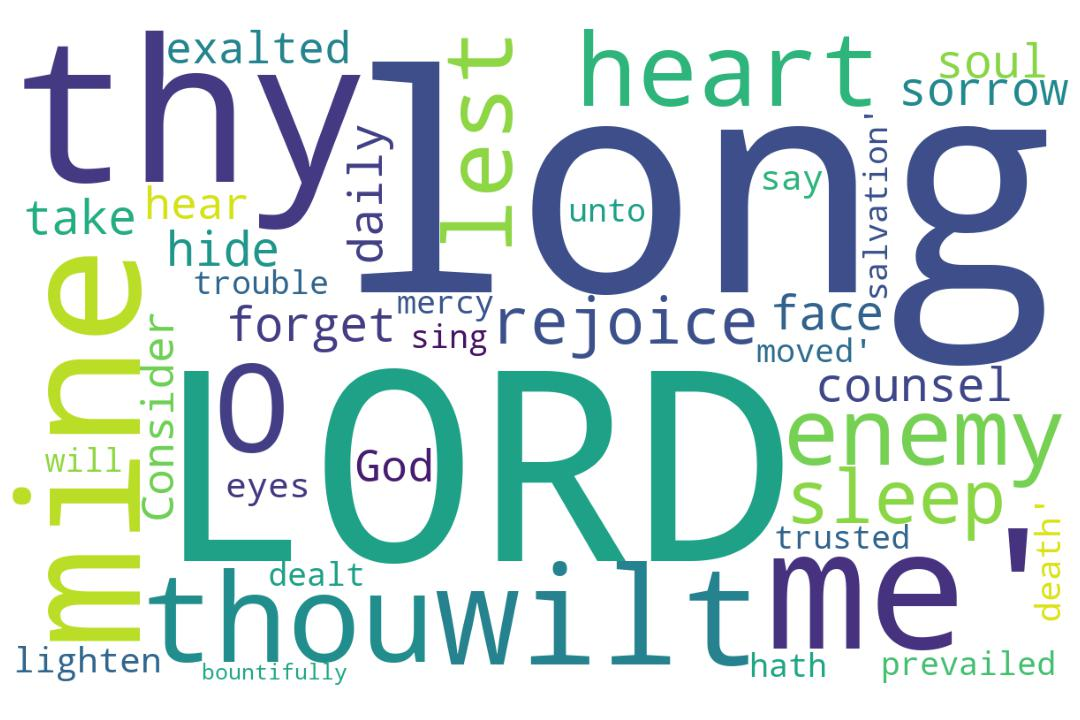
\includegraphics[width=\linewidth]{19OT-Psalms/Psalm13-WordCloud.jpg}
  \caption{Psalm 13 Word Cloud}
  \label{fig:Psalm 13 word Cloud}
\end{figure}


\marginpar{\scriptsize \centering \fcolorbox{bone}{lime}{\textbf{DAVID'S CONTEMPLATION}}\\ (Psalm 13:1-8) 
\begin{compactenum}[I.]
    \item David \textbf{Complains to God} \index[scripture]{Psalms!Psa 013:01}(Psa 13:1)
    \item David \textbf{Confides to God} 
    \item David \textbf{Counsels his Soul}   \index[scripture]{Psalms!Psa 013:02}(Psa 13:2)    
    \item David \textbf{Asks God to Consider him}   \index[scripture]{Psalms!Psa 013:03}(Psa 13:3)
    \item David \textbf{Compares Himself and his Enemies} \index[scripture]{Psalms!Psa 013:04}(Psa 13:4)
    \item David \textbf{Expresses Confidence in God}
    \item David \textbf{Becomes Content with God} \index[scripture]{Psalms!Psa 013:05}(Psa 13:5)
    \item David \textbf{Takes Comfort in God}  \index[scripture]{Psalms!Psa 013:05}(Psa 13:5)%    \item David \textbf{Corrects his Misgivings of God}  \index[scripture]{Psalms!Psa 013:06}(Psalm 13:6)
\end{compactenum}}

\marginpar{\scriptsize \centering \fcolorbox{bone}{yellow}{\textbf{A SONG IN THE HEART}}\\ (Psalm 13:1-8) 
\begin{compactenum}[I.]
    \item The \textbf{Soul} \index[scripture]{Psalms!Psa 013:02}(Psa 13:2)%
    \item The \textbf{Sorrows} \index[scripture]{Psalms!Psa 013:02}(Psa 13:2)%
    \item The \textbf{Supplication} \index[scripture]{Psalms!Psa 013:03}(Psa 13:3)%
    \item The \textbf{Salvation}  \index[scripture]{Psalms!Psa 013:05}(Psa 13:5)%
    \item The \textbf{Satisfaction}  \index[scripture]{Psalms!Psa 013:06}(Psa 13:6)%
    \item The \textbf{Songs} \index[scripture]{Psalms!Psa 013:06}(Psa 13:6)%
\end{compactenum}}

\footnote{\textcolor[cmyk]{0.99998,1,0,0}{\hyperlink{TOC}{Return to end of Table of Contents.}}}\footnote{\href{https://www.audioverse.org/english/audiobibles/books/ENGKJV/O/Ps/1}{\textcolor[cmyk]{0.99998,1,0,0}{Psalms Audio}}}\textcolor[cmyk]{0.99998,1,0,0}{To the chief Musician, A Psalm of David.} %\footnote{John Phillips, How Long? How Long? How Long?:\begin{compactenum}[I.][3]\item Sorrow (Psalm 13:1-2)\item Suplication (Psalm 13:3-4)\item Song  (Psalm 13:5-6)\end{compactenum} } 
\textcolor[cmyk]{0.99998,1,0,0}{\fcolorbox{bone}{lime}{How long} wilt thou forget me, O LORD? for ever? how long wilt thou hide thy face from me?}\footnote{\textbf{Deuteronomy 31:17} - Then my anger shall be kindled against them in that day, and I will forsake them, and I will hide my face from them, and they shall be devoured, and many evils and troubles shall befall them; so that they will say in that day, Are not these evils come upon us, because our God is not among us?}\footnote{\textbf{Job 13:24} - Wherefore hidest thou thy face, and holdest me for thine enemy?}
[2] \textcolor[cmyk]{0.99998,1,0,0}{How long shall I take \fcolorbox{bone}{lime}{counsel} in my soul, \emph{having} sorrow in my heart daily? how long shall mine enemy be exalted over me?}
[3] \textcolor[cmyk]{0.99998,1,0,0}{\fcolorbox{bone}{lime}{Consider} \emph{and} hear me, O LORD my God: lighten mine eyes, lest I sleep the \emph{sleep} \emph{of} death;}
[4] \textcolor[cmyk]{0.99998,1,0,0}{\fcolorbox{bone}{lime}{Lest mine enemy} say, I have prevailed against him; \emph{and} those that trouble me rejoice when I am moved.}\footnote{\textbf{Psalm 3:1} -  LORD, how are they increased that trouble me! many are they that rise up against me.}
[5] \textcolor[cmyk]{0.99998,1,0,0}{But I have trusted in thy mercy; my \fcolorbox{bone}{lime}{heart shall rejoice} in thy salvation.}
[6] \textcolor[cmyk]{0.99998,1,0,0}{\fcolorbox{bone}{lime}{I will sing} unto the LORD, because he hath dealt bountifully with me.}\footnote{\textbf{Psalm 116:7} - Return unto thy rest, O my soul; for the LORD hath dealt bountifully with thee.}\footnote{\textbf{Psalm 119;17} - Deal bountifully with thy servant, that I may live, and keep thy word.}\footnote{\textbf{Psalm 142:7} - Bring my soul out of prison, that I may praise thy name: the righteous shall compass me about; for thou shalt deal bountifully with me.}\footnote{\textbf{2 Corinthians 9:6} - But this I say, He which soweth sparingly shall reap also sparingly; and he which soweth bountifully shall reap also bountifully.}



